\subsection{Portes, \glsfmtlong{gru} et \glsfmtlong{lstm}}

Pour une grande partie des problèmes d'apprentissage \gls{s2s}, les séquences peuvent être très longues.
Le mémoire à court terme constitue donc un véritable obstacle pour l'utilisation des \glspl{rnn} simples en pratique.
Une approche de le contourner qui a eu un énorme succès expérimental, 
est l'introduction d'un mécanisme de contrôle sur la boucle de rétroaction (Voire Figure~\ref{fig.rnn-gate}).
Ce mécanisme est généralement implémenté avec des \emph{portes},
des unités entraînables qui peuvent réguler le flux d'information dans la couche récurrente.
On parle alors d'un \emph{\gls{rnn} à portes}.
Dans cette section, nous explorons les deux variants les plus utilisés d'\glspl{rnn} à portes :
le \gls{gru} et le \gls{lstm}. 


\begin{figure}[htb]
    \begin{center}
        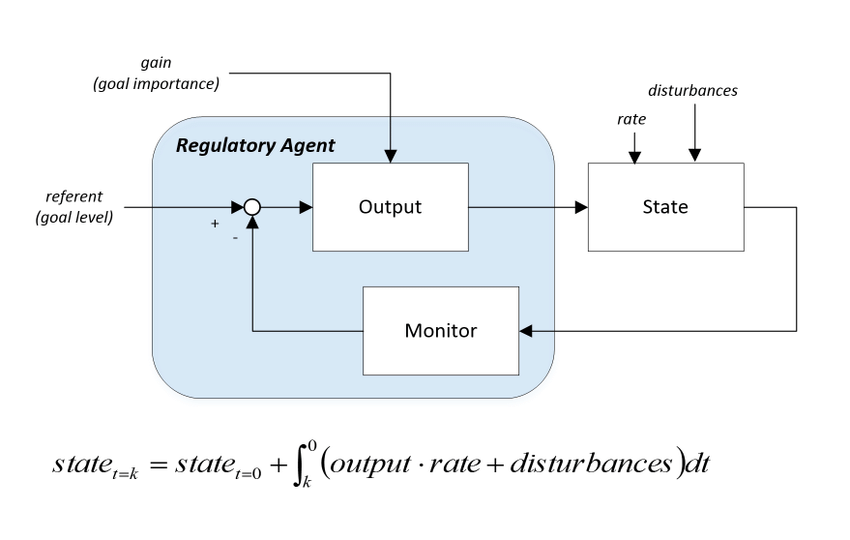
\includegraphics[width=8cm]{gated-feedback.png}
    \end{center}
    \caption{Forme générale d'un \glsfmtshort{rnn} à portes.}
    \label{fig.rnn-gate}
\end{figure}

\subsubsection{\Glsfmtlong{gru}}